
\section{Experiments}



We thoroughly evaluate \ourmethod on a diverse suite of robot embodiments and tasks, testing its ability to generate reward functions, solve new tasks, and incorporate various forms of human input. We use GPT-4~\citep{openai2023gpt4}, in particular the \texttt{gpt-4-0314} variant, as the backbone LLM for all LLM-based reward-design algorithms unless specified otherwise. 

\textbf{Environments.} Our environments consist of 10 distinct robots and 29 tasks implemented using the IsaacGym simulator~\citep{makoviychuk2021isaac}. First, we include 9 original environments from IsaacGym (\textbf{Isaac}), covering a diverse set of robot morphologies from quadruped, bipedal, quadrotor, cobot arm, to dexterous hands. In addition to coverage over robot form factors, we ensure \textit{depth} in our evaluation by including all 20 tasks from the Bidexterous Manipulation (\textbf{Dexterity}) benchmark~\citep{chen2022towards}. Dexterity contains 20 complex bi-manual tasks that require a pair of Shadow Hands to solve a wide range of complex manipulation skills, ranging from object handover to rotating a cup by 180 degrees. For the task description input to \ourmethod, we use the official description provided in the environment repository when possible. See App.~\ref{appendix:environment-details} for details on all environments. It is worth noting that both benchmarks are publicly released concurrently, or after the GPT-4 knowledge cut-off date (September 2021), so GPT-4 is unlikely to have accumulated extensive internet knowledge about these tasks, making them ideal testbeds for assessing \ourmethod's reward generation capability compared to measurable human-engineered reward functions. 






\begin{figure*}[t!]
\centering 
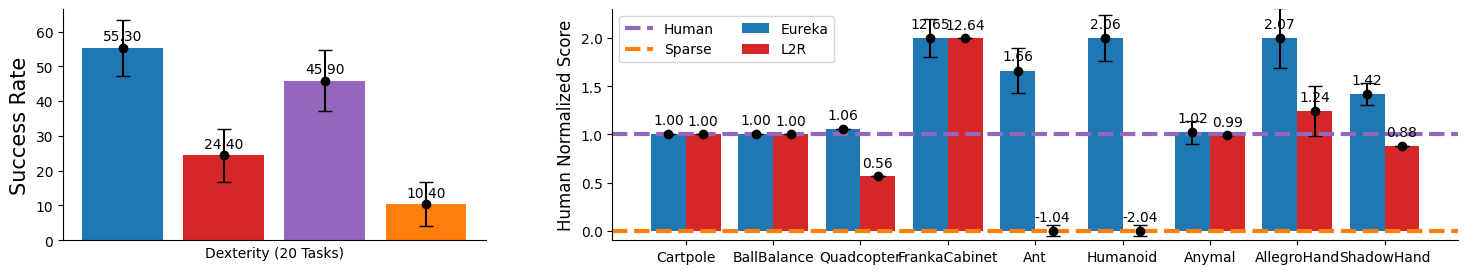
\includegraphics[width=\textwidth]{figures/eureka_bar_chart.png}
\caption{\ourmethod outperforms Human and L2R across all tasks. In particular, \ourmethod realizes much greater gains on high-dimensional dexterity environments.}
  \label{fig:eureka-bar}
\end{figure*}



\subsection{Baselines}

\textbf{L2R}~\citep{yu2023language} proposes a two-stage LLM-prompting solution to generate templated rewards. For an environment and task specified in natural language, a first LLM is asked to fill in a natural language template describing the agent's motion; then, a second LLM is asked to convert this ``motion description'' into code that calls a manually defined set of reward API primitives to write a reward program that sets their parameters. To make L2R competitive for our tasks, we define the motion description template to mimic the original L2R templates, and we construct the API reward primitives using the individual components of the original human rewards when possible. Note that this gives L2R an advantage as it has access to the original reward functions. Consistent with \ourmethod, we conduct 5 independent L2R runs per environment, and for each run, we generate 16 reward samples. See App.~\ref{appendix:baseline-details} for more details.


\textbf{Human.} These are the original shaped reward functions provided in our benchmark tasks. As these reward functions are written by active reinforcement learning researchers who designed the tasks, these reward functions represent the outcomes of expert-level human reward engineering.

\textbf{Sparse.} These are identical to the fitness functions $F$ that we use to evaluate the quality of the generated rewards. Like Human, these are also provided by the benchmark. On the dexterity tasks, they are uniformly binary indicator functions that measure task success; on Isaac tasks, they vary in functional forms depending on the nature of the task. See App.~\ref{appendix:environment-details} for a description of the ground-truth scoring metric for all tasks. 

\subsection{Training Details}
\textbf{Policy Learning.} For each task, all final reward functions are optimized using the same RL algorithm with the same set of hyperparameters. Isaac and Dexterity share a well-tuned PPO implementation~\citep{schulman2017proximal, rl-games2021}, and we use this implementation and the task-specific PPO hyperparameters without any modification. Note that these task hyperparameters are tuned to make the official human-engineered rewards work well. \arxiv{For each final reward function obtained from each method,} we run 5 independent PPO training runs and report the average of the maximum task metric values achieved \arxiv{from 10 policy checkpoints sampled at fixed intervals}. \arxiv{In particular, the maximum is taken over the same number of checkpoints for each approach.}



\textbf{Reward Evaluation Metrics.} For Isaac tasks, since the task metric $F$ for each task varies in semantic meaning and scale, we report the \textbf{human normalized score} for \ourmethod and L2R, $\frac{\texttt{Method} - \texttt{Sparse}}{\lvert \texttt{Human} - \texttt{Sparse} \rvert}$. This metric provides a holistic measure of how \ourmethod rewards fare against human-expert rewards with respect to the ground-truth task metric. For Dexterity, since all tasks are evaluated using the binary success function, we directly report success rates.


\subsection{Results}
\textbf{\ourmethod outperforms human rewards.} In Figure~\ref{fig:eureka-bar}, we report the aggregate results on Dexterity and Isaac. Notably, \ourmethod exceeds or performs on par to human level on \textit{all} Isaac tasks and 15 out of 20 tasks on Dexterity (see App.~\ref{appendix:additional-results} for a per-task breakdown). In contrast, L2R, while comparable on low-dimensional tasks (e.g., CartPole, BallBalance), lags significantly behind on high-dimensional tasks. Despite being provided access to some of the same reward components as Human, L2R still underperforms \ourmethod after its initial iteration, when both methods have had the same number of reward queries. As expected, L2R's lack of expressivity severely limits its performance. In contrast, \ourmethod generates free-form rewards from scratch without any domain-specific knowledge and performs substantially better. \arxiv{In App.~\ref{appendix:additional-results}, we present results on additional evaluation metrics such as interquantile mean (IQM), probability of improvement~\citep{agarwal2021deep}, and the aggregate RL training curves; on all evaluations, we observe the consistent trend that \ourmethod generates the most capable reward functions.} Furthermore, we ablate GPT-4 with GPT-3.5 and find \ourmethod degrades in performance but still matches or exceeds human-level on most Isaac tasks, indicating that its general principles can be readily applied to coding LLMs of varying qualities.




\begin{wrapfigure}{r}{0.6\textwidth}
\centering 
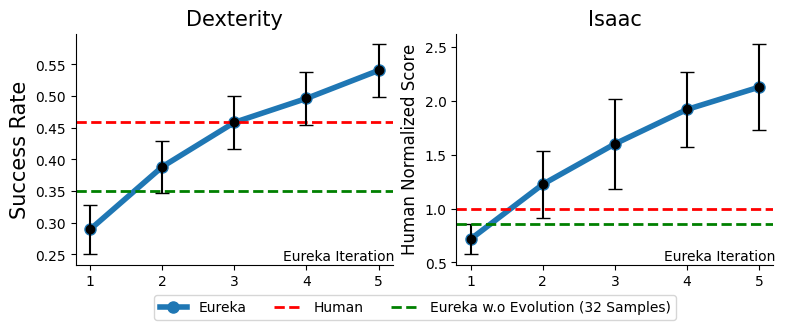
\includegraphics[width=0.6\textwidth]{figures/eureka_improvement.png}
\caption{\ourmethod progressively produces better rewards via in-context evolutionary reward search.}
\vspace{-0.3cm}
  \label{fig:eureka-improvement}
\end{wrapfigure}

\textbf{\ourmethod consistently improves over time.} 
In Fig.~\ref{fig:eureka-improvement}, we 
visualize the average performance of the cumulative best \ourmethod rewards after each evolution iteration. Moreover, we study an ablation, \textbf{\ourmethod w.o. Evolution (32 Samples)}, which performs only the initial reward generation step, sampling the same number of reward functions as two iterations in the original \ourmethod. This ablation helps study, given a fixed number of reward function budget, whether it is more advantageous to perform the \ourmethod evolution or simply sample more first-attempt rewards without iterative improvement. As seen, on both benchmarks, \ourmethod rewards steadily improve and eventually surpass human rewards in performance despite sub-par initial performances. This consistent improvement also cannot be replaced by just sampling more in the first iteration as the ablation's performances are lower than \ourmethod after 2 iterations on both benchmarks. Together, these results demonstrate that \ourmethod's novel evolutionary optimization is indispensable for its final performance. 



\begin{wrapfigure}{r}{0.4\textwidth}
\centering 
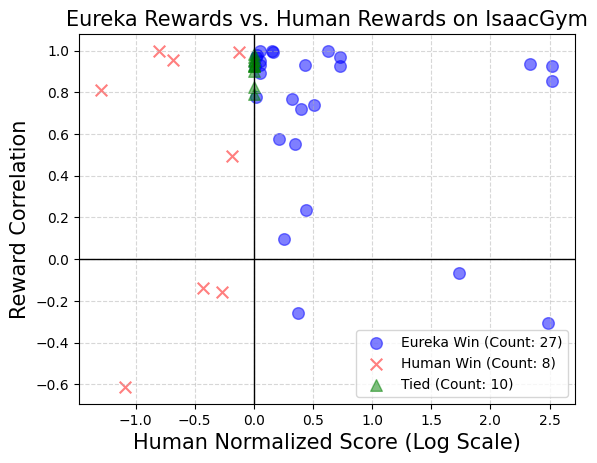
\includegraphics[width=0.4\textwidth]{figures/isaac_eureka_correlation.png}
\vspace{-0.5cm}
\caption{Eureka generates novel rewards.}
  \label{fig:eureka-correlation}
\end{wrapfigure}

\textbf{\ourmethod generates novel rewards.} 
We assess the novelty of \ourmethod rewards by computing the \textit{correlations} between \ourmethod and human rewards on all the Isaac tasks; see App.~\ref{appendix:environment-details} for details on this procedure. Then, we plot the correlations against the human normalized scores on a scatter-plot in Figure~\ref{fig:eureka-correlation}, where each point represents a single \ourmethod reward on a single task. As shown, \ourmethod mostly generates weakly correlated reward functions that outperform the human ones. In addition, by examining the average correlation by task (App.~\ref{appendix:additional-results}), we observe that \textit{the harder the task is, the less correlated the \ourmethod rewards}. We hypothesize that human rewards are less likely to be near optimal for difficult tasks, leaving more room for \ourmethod rewards to be different and better. In a few cases, \ourmethod rewards are even \textit{negatively} correlated with human rewards but perform significantly better, demonstrating that \ourmethod can \textit{discover} novel reward design principles that may run counter to human intuition; we illustrate these \ourmethod rewards in App.~\ref{appendix:negative-correlated-examples}.

\textbf{Reward reflection enables targeted improvement.} 
To assess the importance of constructing reward reflection in the reward feedback, we evaluate an ablation, \textbf{\ourmethod (No Reward Reflection)}, which reduces the reward feedback prompt to include only snapshot values of the task metric $F$. Averaged over all Isaac tasks, \ourmethod without reward reflection reduces the average normalized score by 28.6\%; in App.~\ref{appendix:additional-results}, we provide detailed per-task breakdown and observe much greater performance deterioration on higher dimensional tasks. To provide qualitative analysis, in App.~\ref{appendix:reward-reflection-examples}, we include several examples in which \ourmethod utilizes the reward reflection to perform targeted reward editing.




\textbf{\ourmethod with curriculum learning enables dexterous pen spinning.} 
Finally, we investigate whether \ourmethod can be used to solve a truly novel and challenging dexterous task. To this end, we propose pen spinning as a test bed. This task is highly dynamic and requires a Shadow Hand to continuously rotate a pen to achieve some pre-defined spinning patterns for as many cycles as possible; \arxiv{we implement this task on top of the original Shadow Hand environment in Isaac Gym without changes to any physics parameter, ensuring physical realism.} We consider a \textit{curriculum learning}~\citep{bengio2009curriculum} approach to break down the task into manageable components that can be independently solved by \ourmethod. Specifically, we first use \ourmethod to generate a reward for \arxiv{the task of} re-orienting the pen to random target configurations \arxiv{and train a policy using the final \ourmethod reward}. Then, using this pre-trained policy (\textbf{Pre-Trained}), we fine-tune it using the \arxiv{same} \ourmethod reward to reach the sequence of pen-spinning configurations (\textbf{Fine-Tuned}). To demonstrate the importance of curriculum learning, we also directly train a policy from scratch \arxiv{on the target task} using \ourmethod reward without the first-stage pre-training (\textbf{Scratch}). The RL training curves are shown in Figure~\ref{fig:eureka-pen-spinning}. Eureka fine-tuning quickly adapts the policy to successfully spin the pen for many cycles in a row; see project website for videos. In contrast, neither pre-trained or learning-from-scratch policies can complete even a single cycle of pen spinning. In addition, using this \ourmethod fine-tuning approach, we have also trained pen spinning policies for a variety of different spinning configurations; all pen spinning videos can be viewed on our project website, and experimental details are in App.~\ref{appendix:eureka-pen-spinning}. These results demonstrate \ourmethod's applicability to advanced policy learning approaches, which are often necessary for learning very complex skills



\begin{wrapfigure}{r}{0.4\textwidth}
\centering 
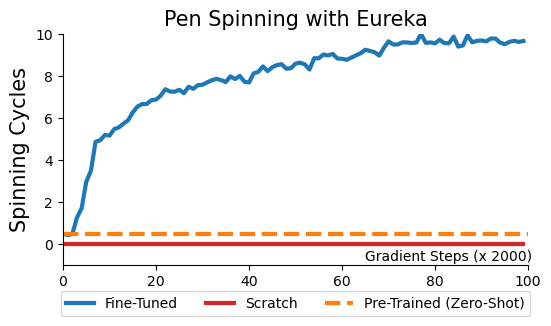
\includegraphics[width=0.4\textwidth]{figures/eureka_pen_spinning.png}
\caption{\ourmethod can be flexibly combined with curriculum learning to acquire complex dexterous skills.}
\vspace{-0.5cm}
  \label{fig:eureka-pen-spinning}
\end{wrapfigure}

















\subsection{\ourmethod From Human Feedback}
\label{sec:eureka-human-feedback}
In addition to automated reward design, \ourmethod enables a new gradient-free in-context learning approach to RL from Human Feedback (RLHF) that can readily incorporate various types of human inputs to generate more performant and human-aligned reward functions.








\textbf{\ourmethod can improve and benefit from human reward functions.} We study whether starting with a human reward function initialization, a common scenario in real-world RL applications, is advantageous for \ourmethod. Importantly, incorporating human initialization requires no modification to \ourmethod\ -- we can simply substitute the raw human reward function as the output of the first \ourmethod iteration. To investigate this, we select several tasks from Dexterity that differ in the relative performances between the original \ourmethod and human rewards. The full results are shown in Figure~\ref{fig:eureka-initialization}.

\begin{wrapfigure}{r}{0.5\textwidth}
\centering 
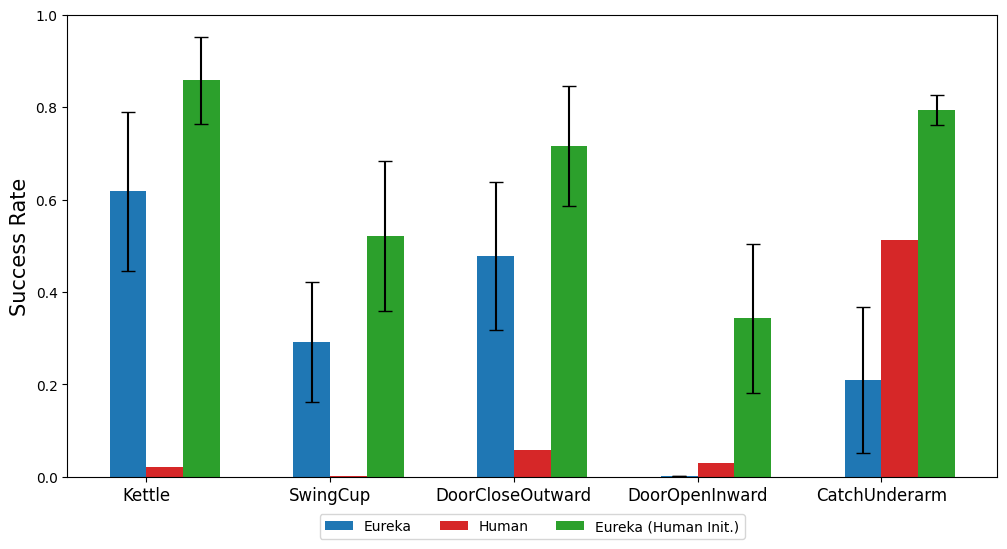
\includegraphics[width=0.5\textwidth]{figures/bidex_reward_assistant.png}
\caption{\small{\ourmethod effectively improves and benefits from human reward initialization.}}
  \label{fig:eureka-initialization}
\end{wrapfigure}

As shown, regardless of the quality of the human rewards, \ourmethod improves and benefits from human rewards as \textbf{\ourmethod (Human Init.)} is uniformly better than both \ourmethod and Human on all tasks. This suggests that \ourmethod's in-context reward improvement capability is largely independent of the quality of the base reward. Furthermore, the fact that \ourmethod can significantly improve over human rewards even when they are highly sub-optimal hints towards an interesting hypothesis: \textit{human designers are generally knowledgeable about relevant state variables but are less proficient at designing rewards using them}. This makes intuitive sense as identifying relevant state variables that should be included in the reward function involves mostly common sense reasoning, but reward design requires specialized knowledge and experience in RL. Together, these results demonstrate \ourmethod's \textit{reward assistant} capability, perfectly complementing human designers' knowledge about useful state variables and making up for their less proficiency on how to design rewards using them. In App.~\ref{appendix:human-initialization-examples}, we provide several examples of \ourmethod (Human Init.) steps.





\textbf{Reward reflection via human feedback induces aligned behavior.} So far, all \ourmethod rewards are optimized against a fixed, black-box task fitness function $F$. This task metric, however, may not fully align with human intent. Moreover, in many open-ended tasks, $F$ may not be available in the first place~\citep{fan2022minedojo}. In these challenging scenarios, we propose to augment \ourmethod by having humans step in and put into words the reward reflection in terms of the desired behavior and correction. We investigate this capability in \ourmethod by teaching a Humanoid agent how to run purely from textual reward reflection; in App.~\ref{appendix:human-reward-reflection-example}, we show the exact sequence of human feedback and \ourmethod rewards. Then, we conduct a user study asking 20 unfamiliar users to indicate their preferences between two policy rollout videos shown in random order, one trained with human reward reflection (\textbf{\ourmethod-HF}) and the other one trained with the original best \ourmethod reward; the details are in App.~\ref{appendix:eureka-rlhf-details}. As shown in Fig.~\ref{fig:eureka-rlhf}, despite running a bit slower, the \ourmethod-HF agent is preferred by a large majority of our users. Qualitative, we indeed see that the \ourmethod-HF agent acquires safer and more stable gait, as instructed by the human. See the project website for a comparison.


\begin{wrapfigure}{r}{0.5\textwidth}
\centering 

\includegraphics[width=0.5\textwidth]{figures/eureka_rlhf.png}
\vspace{0.2cm}
\resizebox{0.5\textwidth}{!}{
\begin{tabular}[c]{l|cc}\toprule
Method & Forward Velocity
& Human Preference \\ \midrule
\ourmethod & \textbf{7.53} & 5/20\\
\ourmethod-HF & 5.58 & \textbf{15/20}\\ 
\bottomrule
\end{tabular}}
\vspace{-0.4cm}
\caption{\ourmethod can incorporate human reward reflection to modify rewards that induce safer and more human-aligned behavior.}
  \label{fig:eureka-rlhf}
\end{wrapfigure}


















